\chapter{如何做好迭代回顾} % Introduction chapter suppressed from the table of contents


\hypertarget{ux4eceux9879ux76eeux51b2ux523aux7684ux56deux987eux590dux76d8ux5f00ux59cb}{%
\subsection{从项目冲刺的回顾复盘开始}\label{ux4eceux9879ux76eeux51b2ux523aux7684ux56deux987eux590dux76d8ux5f00ux59cb}}

在回顾复盘现场,测试人员投影了本次迭代的缺陷分析,展示下面两个缺陷分布图
\begin{itemize}
\tightlist
\item
  开发人员排名(最多的排头)
\item
  按模块来区分(最多的排头)
\end{itemize}

团队组长便按照缺陷的严重程度询问每位开发人员 -\/- 是否知道怎么修改?\\
大家都说知道了。组长要求大家提出问题,如果没有问题就准备散会。

我问:大家好,你们有没有兴趣做个小实验。
后面让我们暂时抛开自己本身是什么岗位。
大家一起看看有哪些地方能减少缺陷?

例如,除了按照人员与模块区分。 我们可否把缺陷简单按下面类型分组 :
需求/设计/编码 ?

他们就让测试人员,展示本冲刺发现的34个缺陷,让大家逐一讨论,找出缺陷是源自哪过程
,最后把总数写在在白板上:

%\href{文件:DefectsBySourceScreenshot_2021-09-20_155232.png}{400px}

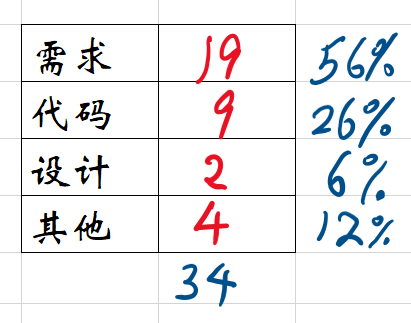
\includegraphics[width=6cm]{DefectsBySourceScreenshot_2021-09-20_155232.png}

让我们看看是怎么分布? 为什么这类缺陷最多呢?大家估计背后是什么原因?
针对需求(最多的类别),我辅导团队利用KJ方法{[}详见附件A2{]},识别主因。最终汇总成以下结果:\\
%\href{文件:!!reqKJfinal微信图片_20210920125228.jpg}{400px}

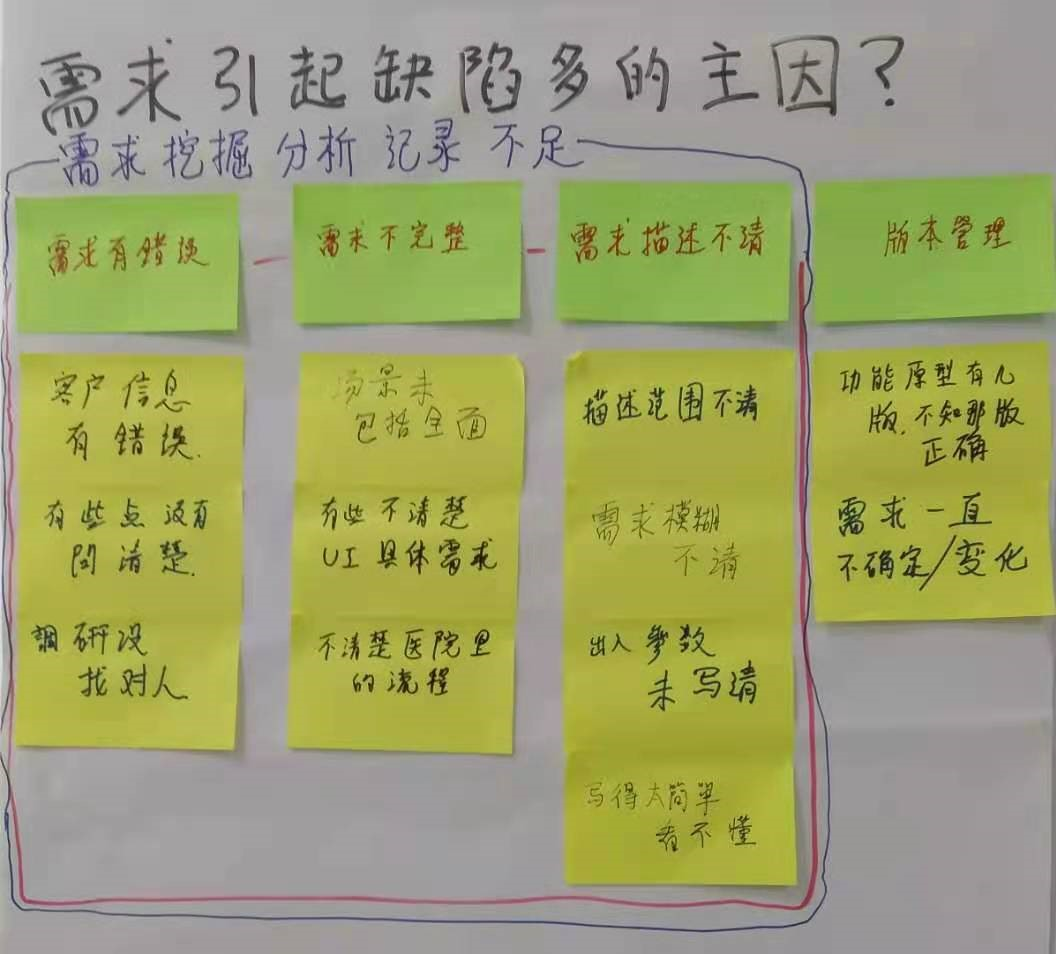
\includegraphics[width=6cm]{reqKJfinal微信图片_20210920125228.jpg}

\hypertarget{ux4eceux95eeux9898ux5206ux6790ux5230ux6839ux672cux539fux56e0ux5230ux884cux52a8}{%
\subsubsection{从问题分析到根本原因到行动}\label{ux4eceux95eeux9898ux5206ux6790ux5230ux6839ux672cux539fux56e0ux5230ux884cux52a8}}

我问:针对我们刚才一起找出的主因,根本原因是什么?
如何可以避免同类缺陷再发生?

答:要加强对需求人员的培训,提高他们的能力。\\
总监说:我年初已察觉到确实很多需求没有表达清楚。
导致开发出来的东西不符合客户要求,或不是客户要的。总监接下来说:

\framebox{%
\begin{minipage}[t]{0.97\columnwidth}\raggedright
我见过以下用户故事:

病人或他的家属能容易找到他选择的服务。\\
理由:他们熟悉网上购物,习惯了方便和快速的响应时间时间。\\
我问需求人员怎样才算容易找到,验收标准?

我估计她记得我说过需求必须可测量,她想了一会,说:验收标准:``普通病人能够在6秒钟内通过不超过三个动作定位任意一项服务。''

我说如果把`普通病人'改为`90\%以上的病人'更好。

必须把模糊,有二义性的需求变成可以测量。

所以不能仅仅说 `新功能很酷,很创新',
而应明确验收标准为:引入了新功能的三个月之内,60\%的用户应该用它来完成规定的工作。75\%以上的用户对产品表示赞许。

所以三个月前,我已经开始 准备正式规划产品经理与需求分析师岗位:
要经过挑选,考试,然后培训,达标才能正式上岗。
本来计划两周后会正式公告,现在既然你们问到,我就预告一下。\strut
\end{minipage}}

我:既然高层已经有长远的规划,我们团队就应该针对下一个冲刺,我们可以做到的事情。\\
团队:我们每个岗位都已经尽了全力,没有什么可以做了。\\
我:你们有做评审吗?如需求,设计评审\\
团队:有。\\
我:需求评审发现多少缺陷,设计评审发现多少?\\
团队:好像两三个。\\
我:发现什么问题?\\
团队:记不清了,当时直接就修改了。\\
我:请问评审总共花了多少时间?多少人参加?\\
团队:我们六个人,那次评审大概用了接近2小时。\\
我:2小时?\\
团队:我们不仅仅发现需求问题,也一起讨论如何修改\\
我:如果评审只找缺陷,记录,应不会超过一小时,如果大家事前做好准备,估计可能半小时可以完成。所以通常检查(Inspection
)不会当场讨论如何修改。\\
我接着说:我们刚才分析系统测试缺陷,不是识别出超过一半是源自需求吗?为什么我们不能在评审时预先发现?你们觉得可以下一个冲刺,评审时可以发现更多缺陷吗?\\
我立马用5分钟与大家分享有效评审能降提高产品质量,降低成本的例子。

团队:估计应该可以,但不知道怎么做?\\
我:你们评审有检查清单吗?\\
团队:没有。\\
我:清单可以帮助我们吸收以往的经验,避免以后同类问题再发生。例如刚才我们都识别了跟需求挖掘/分析/记录不足相关的具体问题吗?
可否利用这些,更新评审检查单的检查项项,提醒我们要避免同类问题。如果大家同意,我们现在就行动。我们要改进便要制定目标,例如计划下次需求评审,系统测试等各过程发现的缺陷数。这些目标你们可以下周一策划两周冲刺时定。

组长安排了小李更新检查单。准备在下次评审前与需求文档,预先发给参评人员。

我:谢谢大家,我没有其他要说了,下次回顾,我或总监会来参加,看看冲刺的效果。

(如想多了解敏捷回顾的流程,详见附件:冲刺回顾与根因分析)

要利用根本原因分析做改进,必须有数据,
也需要有机会立马实验改进方法,评判效果,
所以迭代回顾(或复盘)是做根本原因分析的最佳时机。
但很多团队只在迭代回顾时讨论如何解决迭代暴露的缺陷与相关职责分工,没有探索根本原因,
和如何能避免同类问题再发生。

\hypertarget{ux56deux987eux6d41ux7a0b}{%
\subsection{回顾流程}\label{ux56deux987eux6d41ux7a0b}}

冲刺回顾可按下图的五步,确保各成员都全心投入参与,并能从分析形成行动,达到改进效果:\\
%\#设置舞台 -`破冰'让团队放开顾虑,全心投入讨论 (可参考附件里游戏1)

\begin{enumerate}
\tightlist
\item
  设置舞台 -`破冰'让团队放开顾虑,全心投入讨论 (可参考附件里游戏1)
\item
  收集数据(除了收集`硬'数据,如缺陷,工作量,进度偏差等,也要收集`软'数据,可参考附件里游戏2与3)
\item
  分析,找出根因
  (除了鱼骨图,FMEA,也可参考附件里的KJ分析法,大家利用便利贴做分析)
\item
  决定做什么 (必须明确下个迭代的具体改进行动到人,任务,时间)
\item
  结束
\end{enumerate}

%\href{文件:RetrospectiveScreenshot_2021-09-21_173119.png}{500px}

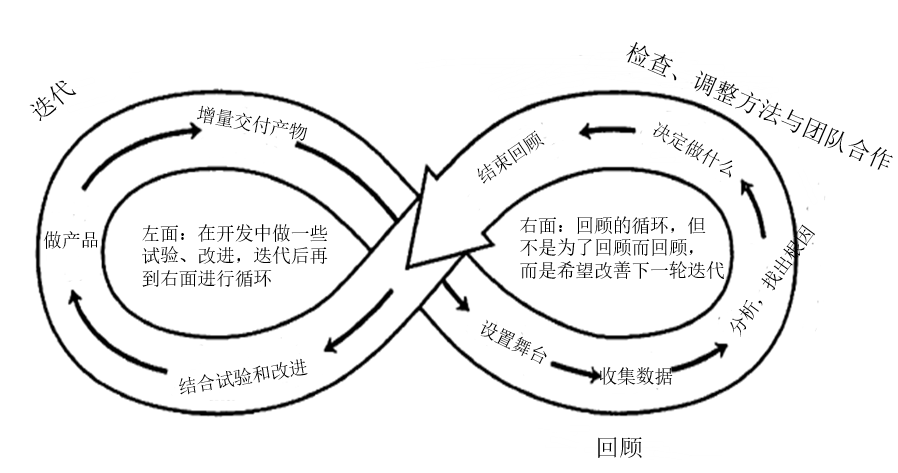
\includegraphics[width=6cm]{RetrospectiveScreenshot_2021-09-21_173119.png}

\hypertarget{ux600eux6837ux5f00ux59cb}{%
\subsection{怎样开始}\label{ux600eux6837ux5f00ux59cb}}

改变人的习惯最困难。
因为团队从未做过这种互动回顾,先利用培训让大家先感受一下,也为收集迭代数据做准备。

建议按以下做模拟互动培训:

%Screenshotfrom2022-12-2921-12-44.png

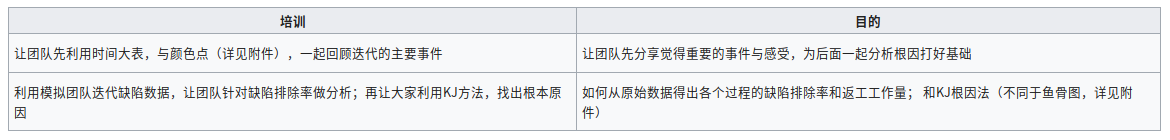
\includegraphics[width=6cm]{Screenshotfrom2022-12-2921-12-44.png}

在游戏1,学员用各种角色扮演什么是吵架,什么是交流,让观众和表演者更能感受到量化回顾先要有对事不对人的心态:

“对话”\\

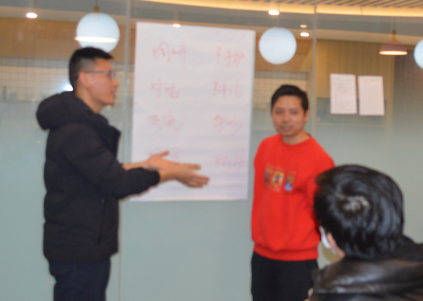
\includegraphics[width=6cm]{1498.png}

“辩论” \\

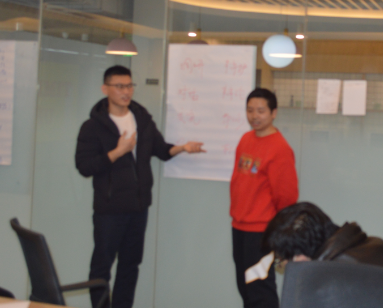
\includegraphics[width=6cm]{1499.png}

\hypertarget{ux5e38ux89c1ux95eeux9898}{%
\subsection{常见问题}\label{ux5e38ux89c1ux95eeux9898}}

\begin{itemize}
\tightlist
\item
  分析只依赖头脑风暴,缺乏数据支撑
\item
  团队没有在迭代收集相关数据
\item
  大家以为是一个问责的讨论会,大家尽力辩护,自己的工作也没有问题,而不能放开共同客观探索过程哪些地方可以改进
\end{itemize}

为什么要做好迭代回顾必须所有干系人参与分析数据,并策划对应的改进行动?

1. 整个团队(所有相关干系人)参与\\
整个团队分析全局问题,避免局部最优(sub-optimization)。例如,如果只是从测试人员的角度,他可能以为缺陷都是来自开发;需求分析人员(或产品经理)会觉得自己做得很好,因需求评审里没有什么问题被发现。但如果团队所有成员聚在一起(包括项目经理、需求、设计、编码、测试),把所有的缺陷列出来,让团队所有岗位一起分析,才可以全局看问题,才可能发现不少问题是因为需求没有明确,导致后面做出来的功能并不是客户要的。后面可扩大参与回顾的干系人,例如客户代表,可以更全面分析。\\
2. 看全局,寻找大家的共通点\\
从Asch
1951实验(详见附件)看到人容易受群众压力影响(尤其当大家不认识),不敢独立表达个人看法,所以很多会议都只是项目经理一言堂,其他人只是观众,没有投入分析。
为了鼓励每人畅所欲言,表达独立看法,并达到共识需要:

\begin{enumerate}
\tightlist
\item
  鼓励每人用实例讲对质量、过程的观点/经验(寻找大家的共通点)
\item
  鼓励每人分享个人感受,想法,满意开心/困惑的时刻(让大家相互了解)
\end{enumerate}

\begin{itemize}
\tightlist
\item
  当大家都感受到面对的问题和情况类似,才会放开自己,分享个人看法
\item
  教练、顾问也鼓励每人发声,大家表达自己的观点
\end{itemize}

所以在我们回顾的时候,也要想办法避免发生这种心理上的影响,导致不能真正挖掘问题的原因。所以在回顾需要大家开放,可以没有压力地畅所欲言。其中一个方式是每人都有水笔+便利贴,找根因讨论时,每人都可以写上自己的意见。而不是传统开会方式,很多时候都只是某一个人讲,其他人听。无法得到每个团队成员的充分参与。如果可以给团队自主权,他们就更能发挥、更能达到目标。\\
最终希望可以全面从每个角色的视角全面分析。

3. 让团队自己寻找改进方案\\

\framebox{%
\begin{minipage}[t]{0.97\columnwidth}\raggedright
必须参与一起分析、讨论,才有动力后面采取行动
\strut
\end{minipage}}
这一点在上章已经说明,并有两个实验验证。

4. 回顾让数据提供者能即时收到反馈\\
%*软件开发与工业生产不一样,大部分的数据必须开发人员自己收集,不能但靠机器/系统(例如:返工工作量)
%因为软件开发是知识性工作,例如,某活动所花的工时,必须靠个人记录(具体步骤可参考以前个人管理)

\begin{itemize}
\tightlist
\item
  软件开发与工业生产不一样,大部分的数据必须开发人员自己收集,不能但靠机器/系统(例如:返工工作量) 因为软件开发是知识性工作,例如,某活动所花的工时,必须靠个人记录(具体步骤可参考以前个人管理)
\item
  但要记录数据要花精力,如果不了解收集的数据,后面有什么用途,便难以维持不断收集数据的习惯
\item
  反之,当大家都清楚到迭代回顾时会一起分析团队数据,并制定针对改进措施,就有动力继续迭代里统计数据
\end{itemize}

\hypertarget{ux5ba2ux6237ux53cdux9988}{%
\subsection{客户反馈}\label{ux5ba2ux6237ux53cdux9988}}

研发总监:
已经做了很多年过程量化考核,起初能给团队带来活力,因为至少比以前好,有路径可以量化他们,员工觉得做有所值,公司也看得见。前几年执行的很好,产出和上线频率比过去好很多。但是现在感觉逐渐拉不出差距来,因为大家都非常熟悉这套游戏规则。

我:理解,比如现在你们团队开始做迭代回顾,团队一起分析根因,持续改善。您觉得效果如何?

研发总监:挺好,但是还是感觉他们开回顾会,耗时太长了,2个小时以上

我:因需要团队收集数据,分析,讨论下迭代措施,所以通常要3小时,熟练后会快一点,底线是改进的节省应大于回顾的投入

\hypertarget{ux603bux7ed3}{%
\subsection{总结}\label{ux603bux7ed3}}

高层的支持是任何改进的重要成功要素。所以首先要让管理者赞同迭代回顾能为公司带来回报(省钱),可以节省的成本(工作量)大于回顾的人力投入;也要让他理解任何改变都有个混沌的过渡期,要经过几轮回顾后,团队才能自己持续改善。下章会分享如何再回顾中利用缺陷排除率与MonteCarlo工具改善大量缺陷都在后面系统测试验收测试才发现的问题,最终能不仅仅降低遗漏到客户的缺陷数,提高质量,也减少工作量(因返工工作量降低),降低开发成本。

\hypertarget{ux9644ux4ef6}{%
\section{附件}\label{ux9644ux4ef6}}


\hypertarget{ux6e38ux620f1ux5e94ux4e0eux5426}{%
\subsection{游戏1:应与否}\label{ux6e38ux620f1ux5e94ux4e0eux5426}}

在迭代回顾中使用。

\hypertarget{ux76eeux7684}{%
\subsubsection{目的}\label{ux76eeux7684}}

帮助建立有效沟通的思维模式。帮助参与者抛开指责和判断,以及对指责和判断的恐惧。

\hypertarget{ux6240ux9700ux7684ux65f6ux95f4}{%
\subsubsection{所需的时间}\label{ux6240ux9700ux7684ux65f6ux95f4}}

8到12分钟,取决于小组的大小。

\hypertarget{ux63cfux8ff0}{%
\subsubsection{描述}\label{ux63cfux8ff0}}

在描述这些模式之后,参与者讨论这些沟通模式的意义。

\hypertarget{ux6b65ux9aa4}{%
\subsubsection{步骤}\label{ux6b65ux9aa4}}

\begin{enumerate}
\tightlist
\item
  将注意力集中在``应与否''(见图4.1),并简要阅读。
\item
  组成小组,每组不超过4人。要求每组用一对词来定义和描述。如果有四对以上的词对/组,如果有多个组有相同的词对,也可以。
\item
  让每个小组讨论他们的两个单词的意思和它们所代表的行为。让他们描述各自对团队和回顾的影响。
\item
  每个小组向整个小组汇报他们的讨论情况。
\item
  询问大家是否愿意使用左面的方式。
\end{enumerate}

\hypertarget{ux6750ux6599ux548cux51c6ux5907}{%
\subsubsection{材料和准备}\label{ux6750ux6599ux548cux51c6ux5907}}

提前准备一张应与否术语的挂图。

%\href{文件:_derby_4.1.png}{500px}

%\includegraphics[width=6cm]{derby_41.png}

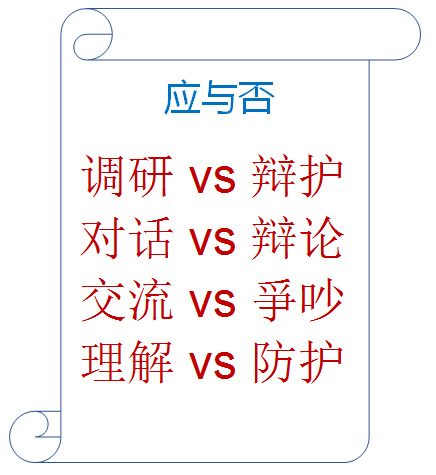
\includegraphics[width=6cm]{Derby_42.png}


调研 vs 辩护\\
对话 vs 辩论\\
交流 vs 爭吵\\
理解 vs 防护\\

\hypertarget{ux6e38ux620f2ux65f6ux95f4ux8868}{%
\subsection{游戏2:时间表}\label{ux6e38ux620f2ux65f6ux95f4ux8868}}

\hypertarget{ux76eeux7684-1}{%
\subsubsection{目的}\label{ux76eeux7684-1}}

促进大家记忆,从多个角度回看之前的工作。大家一起回看谁在什么时候做了什么工作,与当初的假设对比。看是否有什么规律?或者生产水平有没有变化?用来表达事实和每人的感受。

\hypertarget{ux63cfux8ff0-1}{%
\subsubsection{描述}\label{ux63cfux8ff0-1}}

小组成员写卡片来标示那些很有印象、特别有意义或其他重要事件,然后按时间顺序贴在时间表
(Timeline)上。教练鼓励团队讨论事件,以了解已发生的事实和感受。

\hypertarget{ux6b65ux9aa4-1}{%
\subsubsection{步骤}\label{ux6b65ux9aa4-1}}

\begin{enumerate}
\tightlist
\item
  准备时说:``我们希望能够从多个角度来回顾,所以大家每人都要投入,贡献,最终才能让大家真正看到刚结束迭代的全貌。``
\item
  如果总人数多,将团队分成小组,一组不超过5人。保持密切合作的人在一起。尽量分成小组总比合成一个大组好。

  \begin{description}
  \item[]
  分发水笔和卡片(便利贴)。

  确保每人手上都有一支笔。提醒大家要写字清楚,这样大家才能读懂卡片。
  \end{description}
\item
  描述这个过程。

  \begin{description}
  \item[]
  让每人回想一下刚刚的迭代里所有难忘的、有个人意义的或重要的事件,并把它们写在卡片上。

  提醒大家,关键是大家都会有很多观点,不一定要达到的共识。如果这些观点对某人来说有重大意义,便可。

  告诉大家有十分钟的时间做这个活动。

  如果您使用''颜色点``,解释清楚每种颜色的含义并贴上详细说明。

  提醒大家写字清晰。
  \end{description}
\item
  监控大家的进展情况,如果过了一半时间后,有些人还没有开始写卡片,提醒他们要立马开始。当有些组未及时把写好卡片贴上,请他们尽快贴上。

  \begin{description}
  \item[]
  当所有的卡片被粘上后,请团队沿着时间线走,看看其他人张贴了什么。如有人回忆更多的事件时,可以让她添加新卡片。
  \end{description}
\item
  在分析时间表之前,先休息或吃午饭。
\end{enumerate}

\hypertarget{ux529fux80fdux6027ux6cf3ux9053}{%
\subsubsection{功能性泳道}\label{ux529fux80fdux6027ux6cf3ux9053}}

沿时间轴的背景线纵向绘制行(假设你不打算直接在墙上张贴卡片,然后使用丝带或胶带划分行)。为每个部门或功能做一行。每组只会把他们的卡片放在自己组的泳道里。

\hypertarget{ux6750ux6599ux548cux51c6ux5907-1}{%
\subsubsection{材料和准备}\label{ux6750ux6599ux548cux51c6ux5907-1}}

水笔、卡片或便利贴(8cm x 15cm)、大白纸,泥胶,以便可以移动卡片。
用纸覆盖一面墙作为故事画布。1-2周迭代要有0.5 - 1
米高,2米宽;更长的项目要总宽达到10米-20米,高1-1.5米。
在回顾展开始前,先在墙上贴好纸。
(对于发布或项目,用一些时间标记来准备时间表,比如项目里程碑、月份或季节。)

%\url{文件:Timeline2.0.jpg}

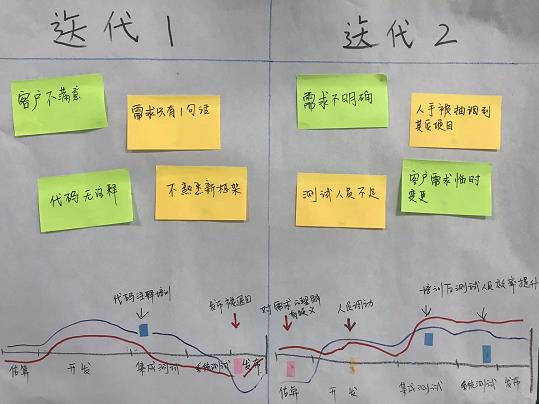
\includegraphics[width=6cm]{Timeline20.jpg}

Figure
5.1:回顾时间表,看着2个迭代。这个团队刚刚开始回顾,所以希望回顾多过一次迭代。

\hypertarget{ux6e38ux620f3ux989cux8272ux70b9}{%
\subsection{游戏3:颜色点}\label{ux6e38ux620f3ux989cux8272ux70b9}}

可与时间表(Timeline)练习结合使用,在更长的迭代回顾中收集团员的感受。

\hypertarget{ux76eeux7684-2}{%
\subsubsection{目的}\label{ux76eeux7684-2}}

展示团队成员对经历事件的感受。

\hypertarget{ux63cfux8ff0-2}{%
\subsubsection{描述}\label{ux63cfux8ff0-2}}

团队成员使用颜色点来表示在时间轴上事件的心情高低。

\hypertarget{ux6b65ux9aa4-2}{%
\subsubsection{步骤}\label{ux6b65ux9aa4-2}}

当所有的事件都已经展示在时间轴上,团队也已经回顾后,每人使用颜色点来显示他们的情绪是高还是低(见图)。

\begin{enumerate}
\tightlist
\item
  ``我们已经一起看了事实,让我们也看看大家工作时的心情,状态。''
  作为开始之前说,让大家理解游戏目的。
\item
  给每个人提供两种颜色的点。每人从7到10个点开始,如后面不够用,可提供更多。解释哪种颜色代表情绪高,哪种颜色代表情绪低。
\item
  让每个人都用点来表示哪里情绪高,哪里停滞、衰弱或低潮。
\end{enumerate}

\hypertarget{ux6750ux6599ux548cux51c6ux5907-2}{%
\subsubsection{材料和准备}\label{ux6750ux6599ux548cux51c6ux5907-2}}

粘点直径为1/2到3/4英寸,有两种颜色。
确定哪种颜色表示高能量,哪种颜色表示低能量。

%\url{文件:便利贴1.jpg}

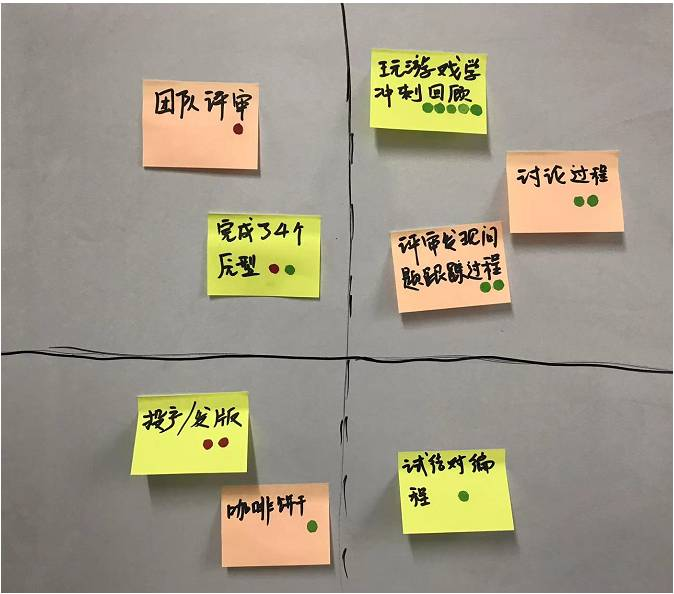
\includegraphics[width=6cm]{便利贴1.jpg}

\hypertarget{asch-1951-ux7fa4ux4f17ux538bux529bux5b9eux9a8c}{%
\subsection{Asch 1951
群众压力实验}\label{asch-1951-ux7fa4ux4f17ux538bux529bux5b9eux9a8c}}

%\href{文件:Asch0Screenshot_2022-07-09_161023.jpg}{150px}

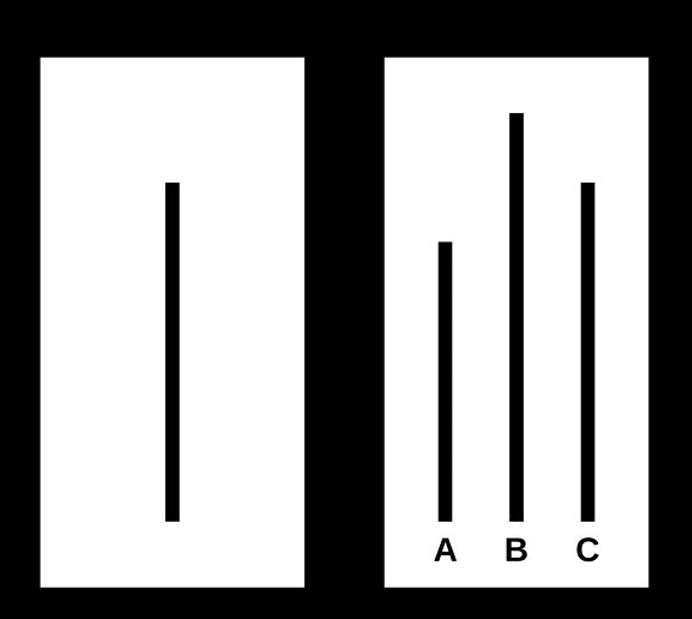
\includegraphics[width=6cm]{Asch0Screenshot_2022-07-09_161023.jpg}

问题:\textbf{请问右面那条线 (A, B, C) 的长度最接近左面线的长度?}

%\url{文件:Asch2Screenshot.jpg}

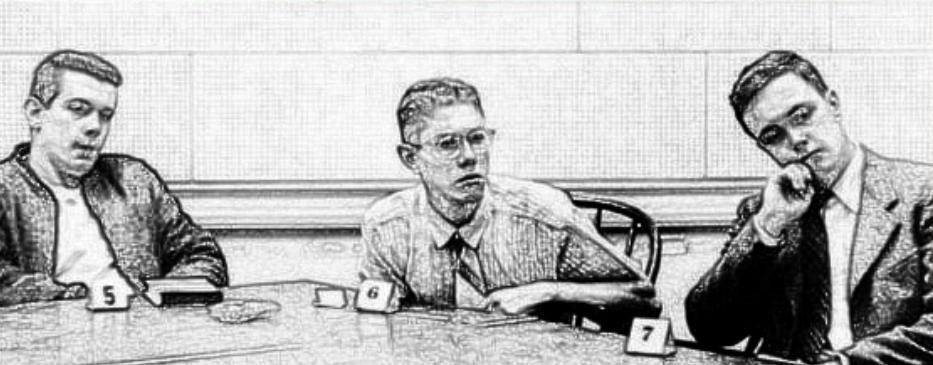
\includegraphics[width=6cm]{Asch2Screenshot2.png}

实验设计:\textbf{随机邀请几位志愿者(包括你)
参加,实验之前与(除了你以外)所有人预先说好,都选A,并且要假装成经过深思熟虑。实验时,你是最后一位作答。}

结果:

\begin{itemize}
\tightlist
\item
  有群众压力时,大概\textbf{37\%}会从众选择错误答案
  (虽然不同人有差异,但总体只有\textbf{25\%}能坚持自己的正确答案。)
\item
  个人自己作答,接近100\%选对,错误率\textbf{少于1\%}
\end{itemize}

影响因素:

\begin{itemize}
\tightlist
\item
  前面选择错误答案的人数越多,错误率越高:
\end{itemize}

\begin{enumerate}
\tightlist
\item
  一位:接近0\%答错
\item
  两位:大概14\%
\item
  三位: 32\%(详见下图)
\end{enumerate}

%\href{文件:Asch3Screenshot_2022-07-08_201341.jpg}{500px}

%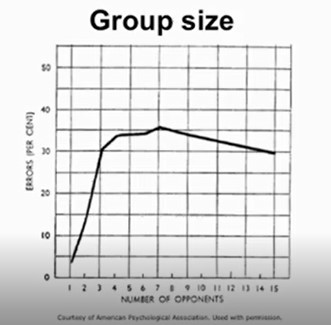
\includegraphics[width=6cm]{Asch3Screenshot_2022-07-08_201341.jpg}


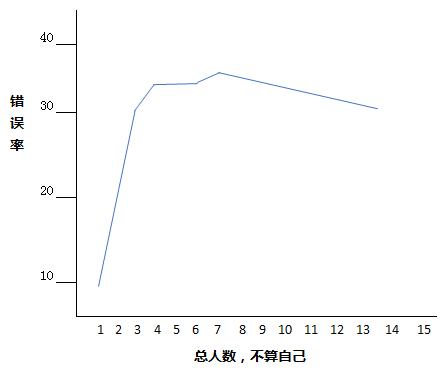
\includegraphics[width=6cm]{Asch3Screenshot_2022-07-08_2013411.png}

\begin{itemize}
\tightlist
\item
  如果前面其中一位选了正确答案,你的错误率就显著降低(大约原本水平的1/4,看下图黄线),并让你感到与他更亲切
\item
  但当这`战友'后面实验里也从众选错误答案,你的错误率会返回原本水平(原本水平是下图绿线)
\end{itemize}

%\href{文件:Asch4Screenshot_2022-07-08_201502.jpg}{500px}

%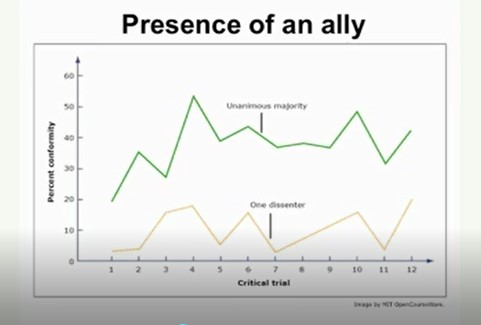
\includegraphics[width=6cm]{Asch4Screenshot_2022-07-08_201502.jpg}

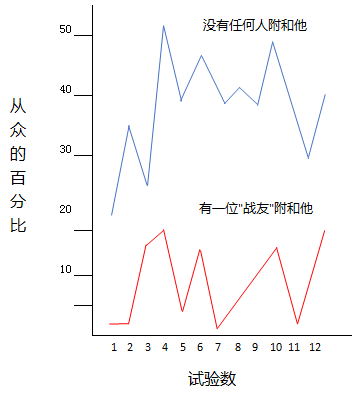
\includegraphics[width=6cm]{Asch4Screenshot_2022-07-08_2015021.png}

\begin{itemize}
\tightlist
\item
  尴尬场景(例如,迟到),你的错误率会更高

  \begin{itemize}
  \tightlist
  \item
    实际你没有晚到,只是让你觉得确实迟到了,觉得尴尬
  \end{itemize}
\item
  如果不是要你说出答案,而是让你把答案写在纸上,错误率会降低三分之一
\end{itemize}

\hypertarget{kjux6b65ux9aa4}{%
\subsection{KJ分析方法步骤}\label{kjux6b65ux9aa4}}

\emph{一种头脑风暴方法,每人把自己想法写在便利贴上,一起轮流把所有便利贴排放分组}

\begin{enumerate}
\tightlist
\item
  把主题以问题形式写在大白纸的头顶;
\item
  把相关的事实写在便利贴上面,用黑色;
\item
  搜集相关的事实,如果是一组人的话,分散到不同人手上;
\item
  (团队)查看描述是否不清楚,是否要整理?
\item
  每人轮流把相关的便利贴组合在一起;
\item
  当每人都已经调整过便利贴组合后,一起把每一组便利贴加上一个题目,用红色标识;
\item
  红色的标题下包含相关事实的内容;
\item
  把相关的红色题目(最好不超过3个)组合在一起;
\item
  给这大组一个题目 -- 蓝色;
\item
  在题目下放上相关的红色小组;
\item
  把蓝色的题目和剩下红色的小组或单独没有分类的便利贴都在墙上放好,也可以用一些箭头描述它们的因果关系;
\item
  (可选)
\end{enumerate}

\begin{description}
\item[]
\begin{description}
\tightlist
\item[]
A: 投票看看哪个是最重要的红色组

B: 也可以加些总结性的描述
\end{description}
\end{description}

%\href{文件:KJ_1.0.png}{600px}

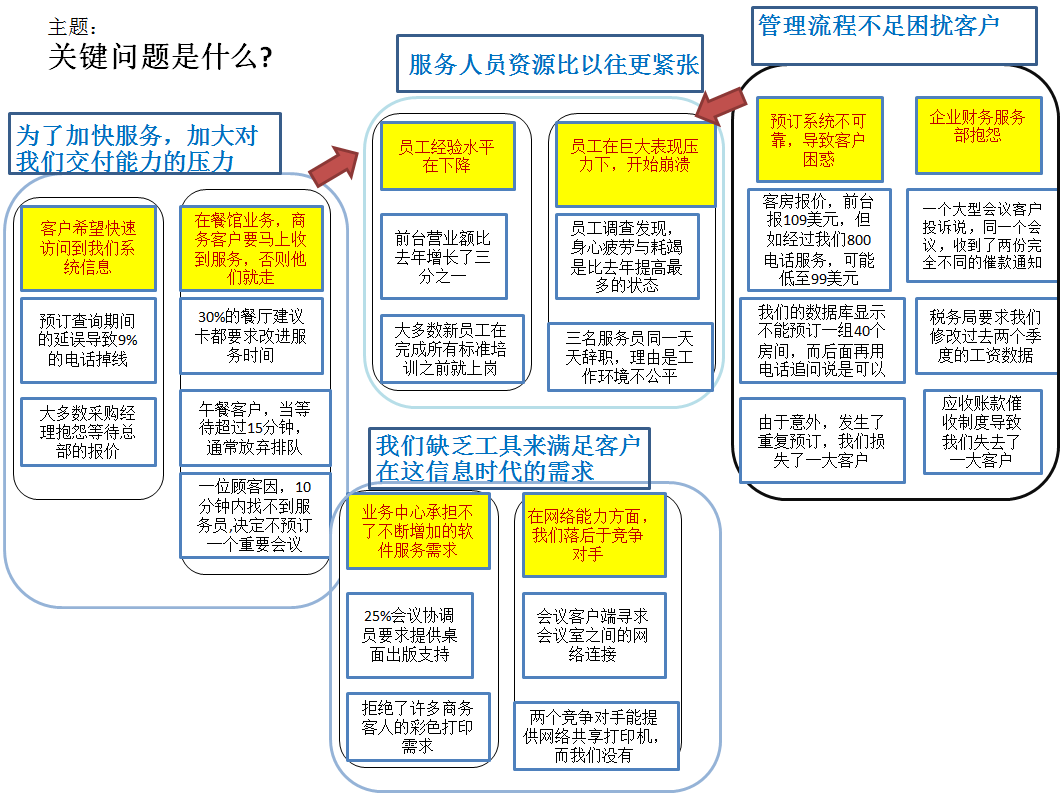
\includegraphics[width=6cm]{KJ_10.png}

\hypertarget{references}{%
\section{References}\label{references}}

1. Derby, E. : Agile Retrospectives: Making Good Teams Great (2006)





